\subsection{Timing}
  In addition to giving a count of floating point operations in our algorithms, we show that they can be implemented as a BLAS library comparable in speed to commercially available optimized non-reproducible versions.

  All timings are performed with an Intel\textregistered Core i7-2600 CPU
  operating at 3.4 GHz with 32 KB L1 Cache, 256 KB L2 Cache, and 8192 KB L3
  Cache. Every test is run at least 100 times successively to amortize the data
  loading time and warm up the cache. The largest BLAS1 problems (sum and dot
  product) were resident in the L2 cache. The largest BLAS2 and BLAS3 problems
  exceeded even the L3 cache size. With the intention that these results may be
  reproduced, we chose to use the widely available open-source compiler
  \texttt{gcc}. The code was compiled with \texttt{gcc} version 4.8.4 using the
  highest level ``\texttt{-O3}'' of optimization (and no other optimization
  flags). We compare our BLAS routines against the sequential
  Intel\textregistered Math Kernel Library (MKL) BLAS Version 11.0.5 routines
  \cite{MKL}. All matrices are represented in column-major order. Denormalized
  floating point arithmetic is known to be much slower than normalized floating
  point arithmetic. It should be noted that for all tests, we do not measure with
  denormal values, as this is the most common case in practice.

  The theoretical peak time is calculated as the idealized theoretical time in
  which the CPU could complete the given operations (in any order). We include the or-bit operation as a FLOP along with multiplication and addition. We
  multiply the peak processing rate by the number of floating point types that
  can be processed in a single vectorized instruction (using SSE or AVX
  intrinsics) \cite{SSEAVX}. Because instructions of differing type (addition,
  multiplication, or or-bit operation) can be completed in parallel on our
  particular CPU, we assume that the peak processing time depends only on the
  maximum number of instructions of a single type. The theoretical peak
  time $t$ is therefore calculated according to \eqref{eq:peak}.
  \begin{align}
    a &= \text{number of additions}\nonumber\\
    m &= \text{number of multiplications}\nonumber\\
    o &= \text{number of or-bit operations}\nonumber\\
    f &= \text{CPU frequency}\nonumber\\
    v &= \text{number of floating-point types that fit into largest supported vector register}\nonumber\\
    t &= \frac{\max(a, m, o)}{vf}
    \label{eq:peak}
  \end{align}

  \subsubsection{Difficult Input}
    Because the reproducible summation algorithm needs to perform additional
    operations (Algorithm \ref{alg:update}) if the maximum absolute value of the
    data increases during summation, the run time depends (up to a constant factor)
    upon the input. To show the differences in run time, we show in Figure
    \ref{fig:easy_vs_hard_timings} the time it takes to reproducibly sum $2^{13}$
    \texttt{double}s and \texttt{float}s from two different data sets. The first
    data set is an easy case, the uniform distribution from 0 to 1. The second data
    set is the most difficult possible case, numbers (alternating in sign to avoid
    infinities) increasing in absolute value exponentially starting at 1 and ending
    with the largest positive finite floating point value. We chose to start this
    increase at 1 rather than the minimum positive floating point value to avoid
    denormalized floating point values. This data set is difficult because the
    exponent of the maximum absolute value increases linearly from 0 to its maximum
    possible value. Therefore, the \textproc{Update} operation (Algorithm
    \ref{alg:update}) must be performed more frequently to adjust the index of the
    indexed type. We can compare this to the uniform distribution in $[0, 1)$,
    which very quickly achieves a number (greater than $0.5$) that has the largest
    floating point exponent possible from the distribution. After such a number is
    seen, no more updates need to be performed. Note that these problems were
    resident in the L2 cache. We calculate the peak performance of \texttt{rxsum}
    using only the core operations in the \textproc{DepositRestricted} operation
    (Algorithm \ref{alg:depositrestricted}). \texttt{rdsum} achieved performance of
    $1.20\cdot 10^{10}$ FLOPS ($61.9\%$ of peak) on the difficult dataset.
    \texttt{rssum} achieved performance of $1.88\cdot 10^{10}$ FLOPS ($48.6\%$ of
    peak) on the difficult dataset. It is clear from the figure that the additional
    cost of the \textproc{Update} operation is modest, and the performance of the
    summation algorithm has only a weak dependence on the data.
  \begin{figure}[H]
  \begin{center}
  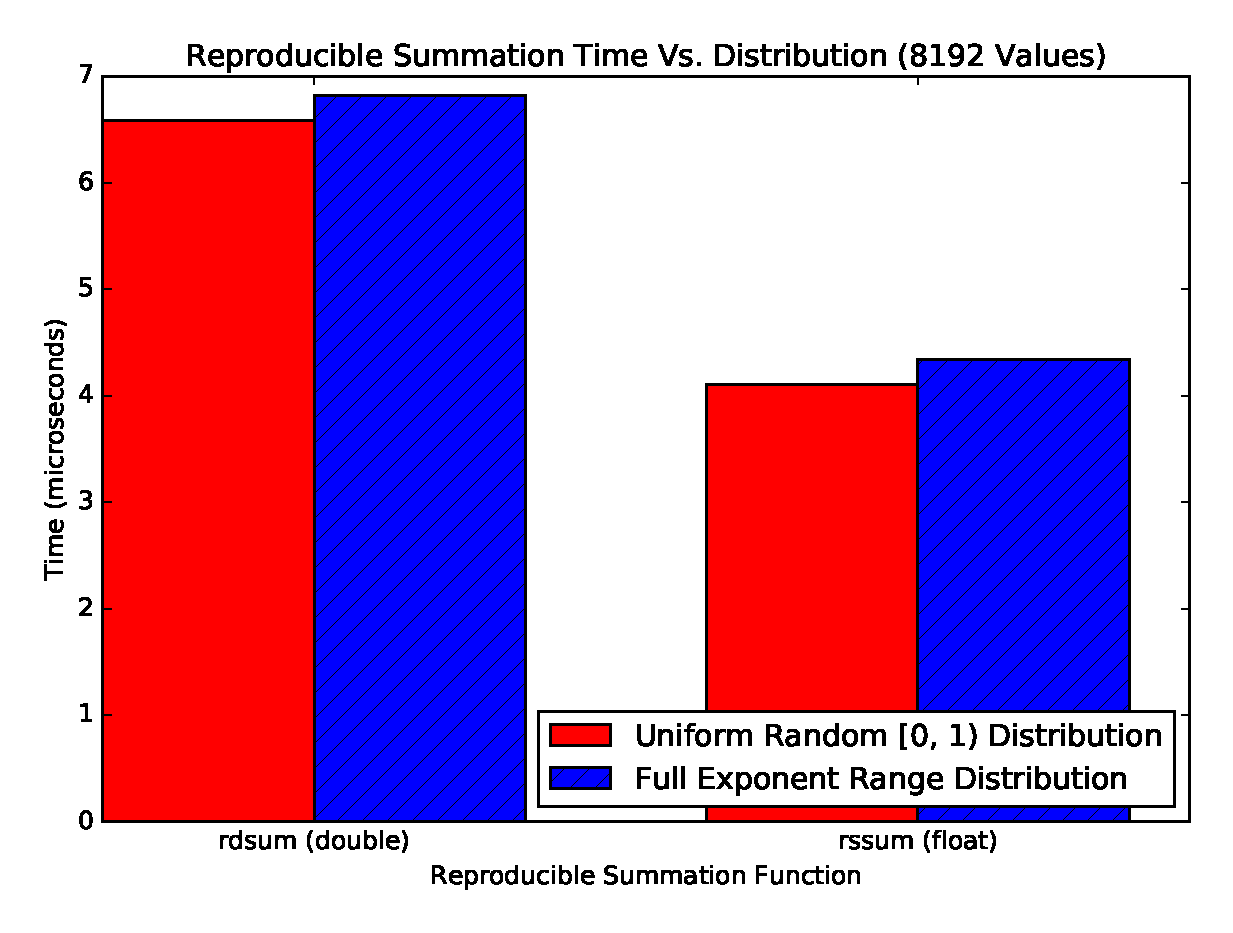
\includegraphics[width=\textwidth]{plots/easy_vs_hard}
  \caption{Time taken to sum $2^{13}$ floating point numbers of varying difficulty.}
  \label{fig:easy_vs_hard_timings}
  \end{center}
  \end{figure}
  \subsubsection{BLAS1}

    We show how our reproducible summation compares to a simple C \texttt{for}-loop in Figure \ref{fig:forloop_timings}. We compiled the \texttt{for}-loop using the command ``\texttt{gcc -03}''. The \texttt{for}-loop is as follows (where \texttt{X} is the input vector and \texttt{res} is the resulting sum):
    \begin{lstlisting}

    res = 0;
    for(j = 0; j < N; j++){
      res += X[j];
    }
    \end{lstlisting}

  Time (measured relative to the peak theoretical time for recursive summation) is shown for each method. The double-precision floating point numbers to be summed are normally distributed with mean $0$ and variance $1$. The values of $N$ shown are powers of two from $2^6$ to $2^{12}$. All of the problems shown on this plot were resident in L1 cache. The peak performance of \texttt{rdsum} is $1.94\cdot 10^{10}$ FLOPS. The peak performance of the \texttt{for}-loop is $1.36\cdot 10^{10}$ FLOPS. The peak performance of the \texttt{for}-loop is $0.7$ times that of \texttt{rdsum}, as the \texttt{for}-loop requires 1 addition per element, but \texttt{rdsum} requires $3K - 2 = 7$ additions and $K = 3$ or-bit operations per element which can be done in parallel. This also explains why the theoretical peak time required for \texttt{rdsum} is 7 times larger than the \texttt{for}-loop. Compiling with the \texttt{gcc} flag \texttt{-fopt-info-vec-optimized} tells us that the \texttt{for}-loop is not vectorized by the compiler, and therefore not running at peak. With this in mind, reproducible summation is competitive with a simple \texttt{for}-loop.
  \begin{figure}[H]
  \begin{center}
  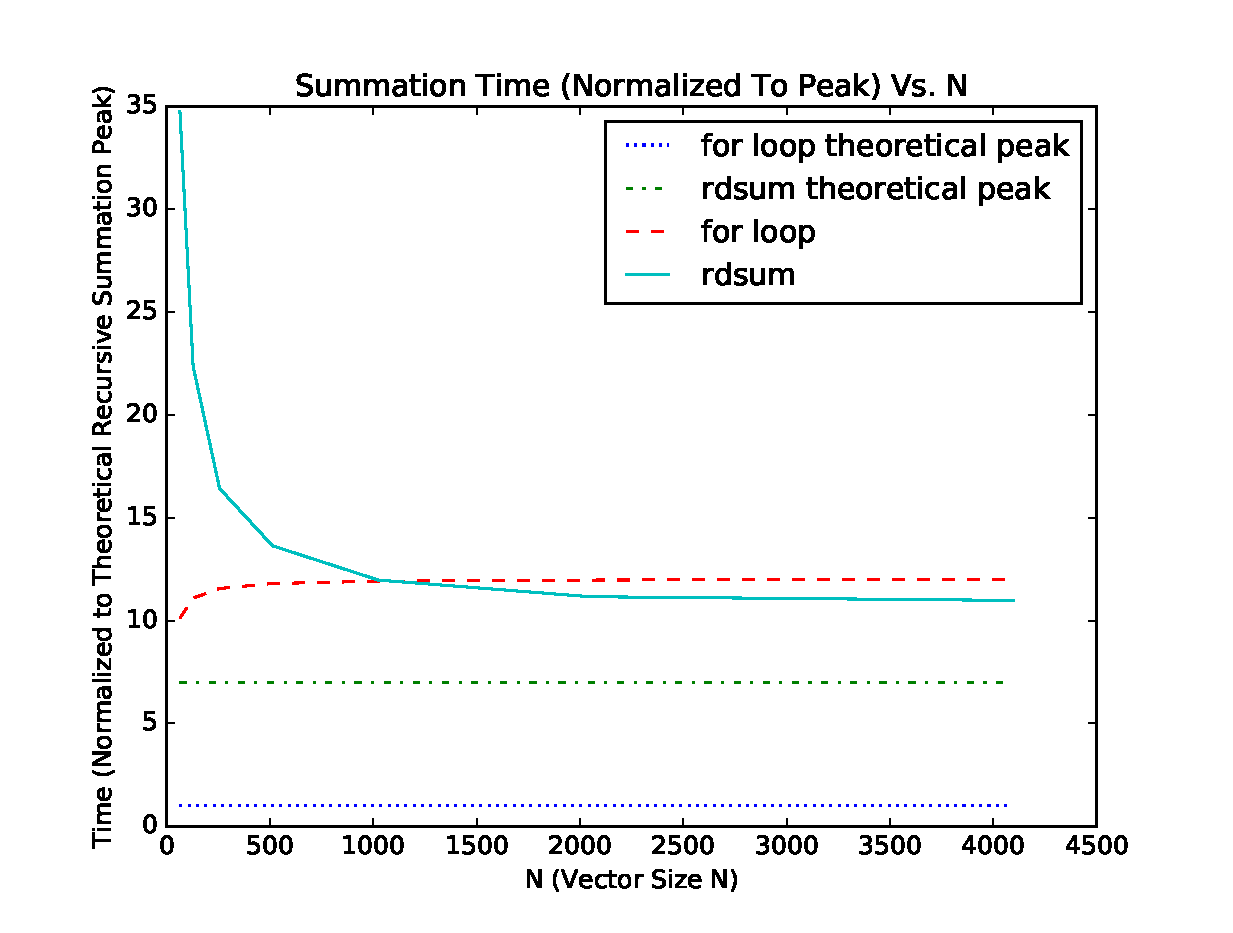
\includegraphics[width=\textwidth]{plots/sum_comparison}
  \caption{Relative floating point summation time}
  \label{fig:forloop_timings}
  \end{center}
  \end{figure}
    To give a comparison to a BLAS1 function, we show in Figure \ref{fig:dot_timings} timings of the reproducible dot product versus the MKL BLAS dot product. Again, the double-precision floating point data is distributed such that the elements of each input vector are normally distributed with mean $0$ and variance $1$. The values of $N$ shown are powers of two from $2^6$ to $2^{12}$. All problems shown here were L1 resident except for the largest problem, which was resident in the L2 cache. We calculate peak performance of \texttt{rddot} using only the core operations in the \textproc{DepositRestricted} operation (Algorithm \ref{alg:depositrestricted}) and the additional pointwise multiplication. The peak performance of \texttt{rddot} is $2.14\cdot 10^{10}$ FLOPS. The peak performance of \texttt{ddot} is $2.72\cdot 10^{10}$ FLOPS. The peak performance of \texttt{ddot} is $1.27$ times that of \texttt{rddot}. This is because \texttt{ddot} requires 1 addition and 1 multiplication per element, while \texttt{rddot} requires $3K - 2 = 7$ additions, 1 multiplication, and $K = 3$ or-bit operations per element. This also explains why the theoretical peak time required for \texttt{rddot} is 7 times larger than that of \texttt{ddot}.
  \begin{figure}[H]
  \begin{center}
  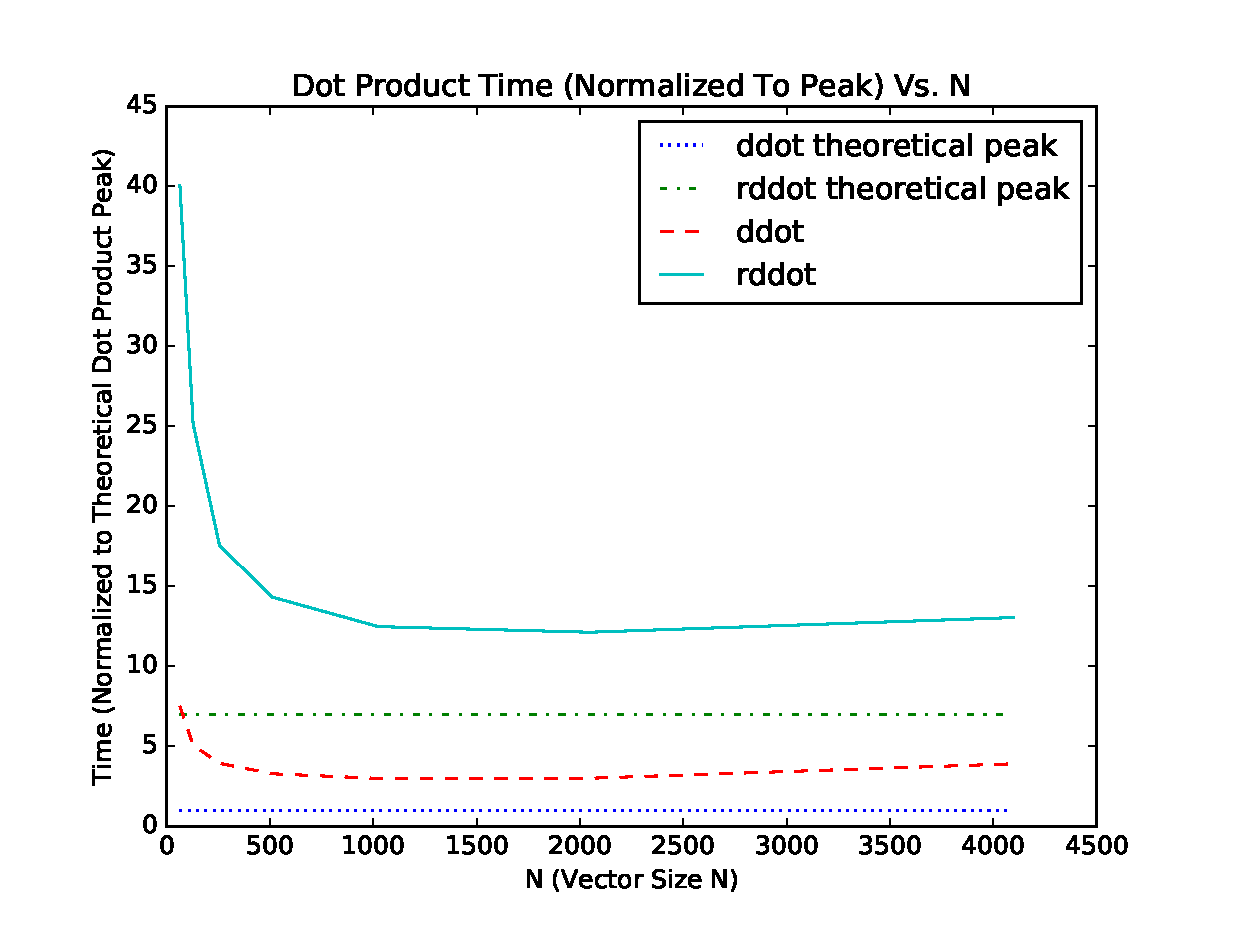
\includegraphics[width=\textwidth]{plots/dot_comparison}
  \caption{Relative dot product time}
  \label{fig:dot_timings}
  \end{center}
  \end{figure}
  \subsubsection{BLAS2}
    We show in Figure \ref{fig:gemv_timings} timings of the reproducible matrix-vector product versus the MKL BLAS matrix-vector product. Each double-precision floating point input matrix or vector element is normally distributed with mean $0$ and variance $1$. The values of $N$ shown are powers of two from $2^6$ to $2^{12}$. Problem size $2^6$ was resident in L1 cache, problem size $2^7$ was resident in L2 cache, problem sizes $2^8$ to $2^{10}$ were resident in L3 cache, and problem sizes $2^{11}$ and $2^{12}$ exceeded the L3 cache size. The peak performances of \texttt{rdgemv} and \texttt{dgemv} are the same as that of \texttt{rddot} and \texttt{ddot}.
  \begin{figure}[H]
  \begin{center}
  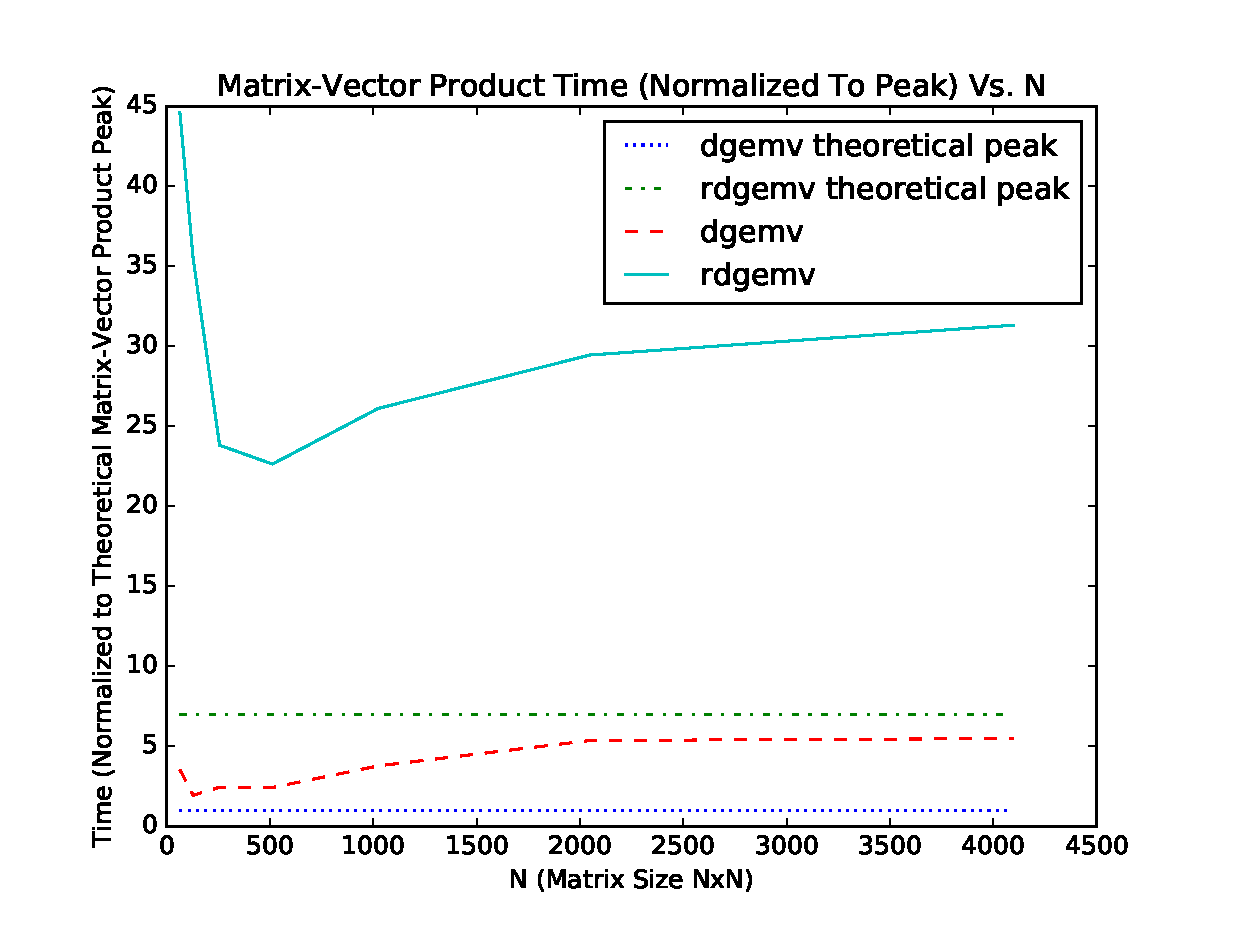
\includegraphics[width=\textwidth]{plots/gemv_comparison}
  \caption{Relative matrix-vector product time}
  \label{fig:gemv_timings}
  \end{center}
  \end{figure}
  The non-transposed matrix-vector product is the only case where composition of BLAS2 and BLAS3 functions did not achieve results within a factor of 2 of theoretical peak. Because the reproducible dot product operates most efficiently on contiguous sections of memory, the matrix must be transposed so that memory can be read contiguously. This causes the reproducible matrix-vector product to perform poorly due to the extra cost of matrix transposition in an already memory-bound routine. In future versions of the library, this method could be improved by writing a custom inner-loop kernel that does not make calls to \texttt{xixdot}. The kernel would operate on the primary fields of several indexed types at the same time using vectorized operations.

  The transposed matrix-vector product performs better than the non-transposed case. Timings are shown in Figure \ref{fig:gemv_trans_timings}. The reader should notice that in this case, the reproducible routine is only a factor of $2.41$ times slower than the optimized BLAS routine.
  \begin{figure}[H]
  \begin{center}
  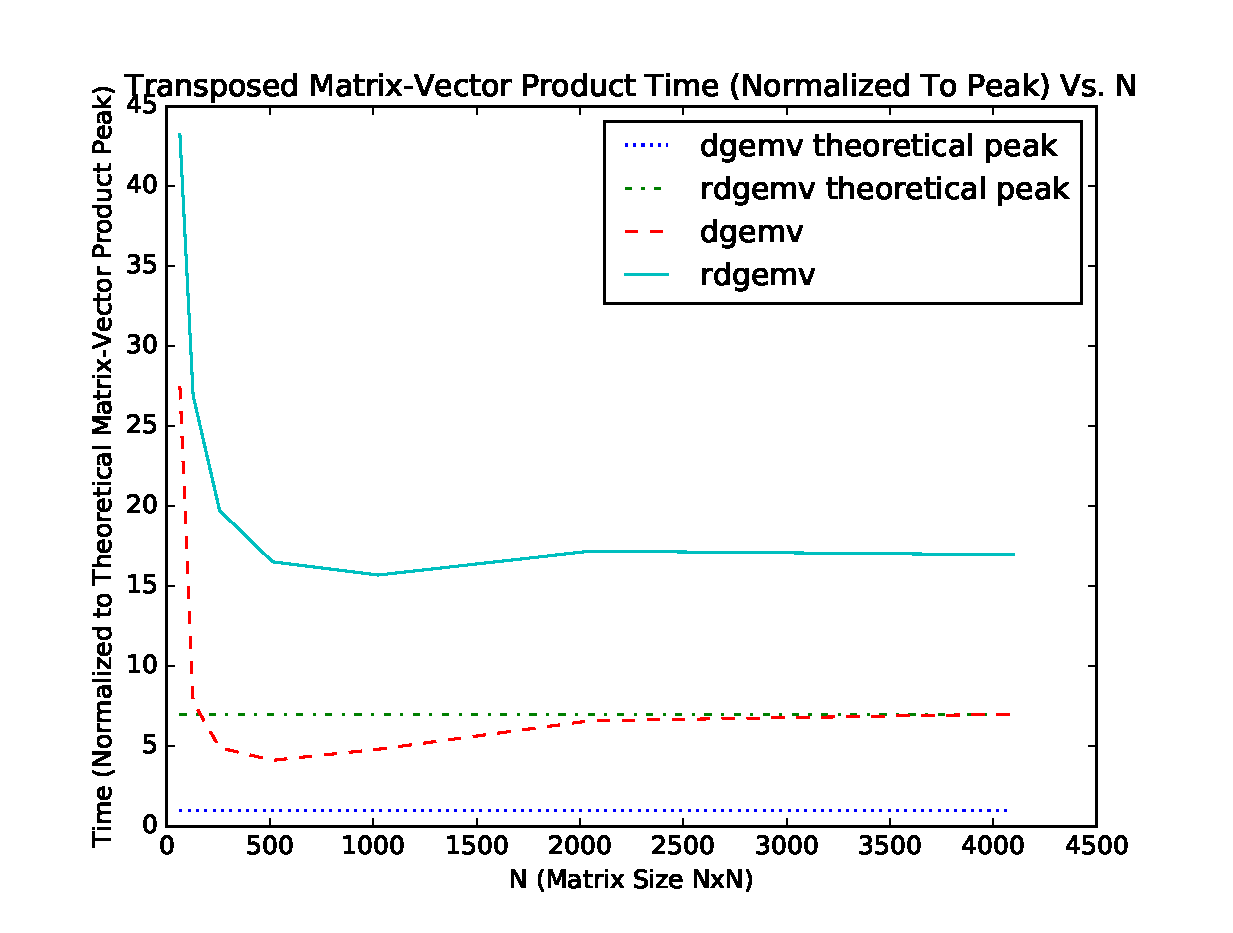
\includegraphics[width=\textwidth]{plots/gemv_trans_comparison}
  \caption{Relative transposed matrix-vector product time}
  \label{fig:gemv_trans_timings}
  \end{center}
  \end{figure}

  \subsubsection{BLAS3}
    We show in Figure \ref{fig:gemm_timings} timings of the reproducible matrix-matrix product versus the MKL BLAS matrix-matrix product. Because the timings for each transposition case (transposing or not transposing $A$ or $B$) are similar, we show only the standard case for brevity. Each double-precision floating point input matrix element is normally distributed with mean $0$ and variance $1$. The values of $N$ shown are powers of two from $2^6$ to $2^{12}$. Problem size $2^6$ was resident in L2 cache, problem sizes $2^7$ to $2^9$ were resident in L3 cache and problem sizes $2^{10}$ to $2^{12}$ exceeded the L3 cache size. The peak performances of \texttt{rdgemm} and \texttt{dgemm} are the same as that of \texttt{rddot} and \texttt{ddot}. In this case, since \texttt{dgemm} is running close to peak and \texttt{rdgemm} is running at about half of peak, the reproducible routine is a factor of $12.8$ times slower than the optimized BLAS routine.
  \begin{figure}[H]
  \begin{center}
  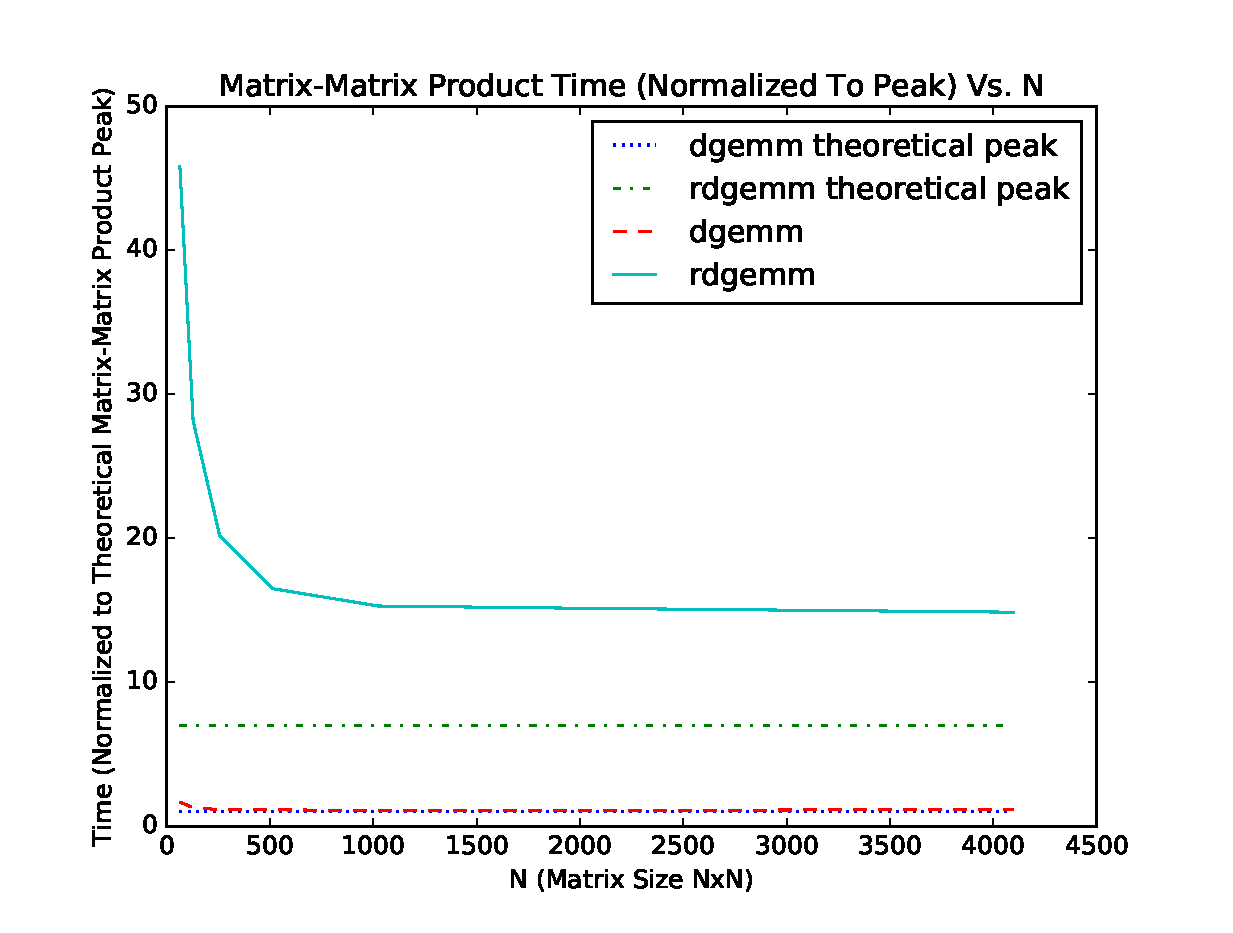
\includegraphics[width=\textwidth]{plots/gemm_comparison}
  \caption{Relative matrix-matrix product time}
  \label{fig:gemm_timings}
  \end{center}
  \end{figure}
